\section{Equilibrium transition experiments}
\label{sec:numerical}

Every path reported in this section solves the decentralized perfect-foresight
canonical system on its reported interval. The numerical solution imposes the household Euler equation, the
developer's research first-order and costate conditions, monopoly supply of AI
services, labor-market clearing, and the aggregate resource constraint. Earlier
experiments that fixed investment and automated-research spending as shares of
output are retained in the replication files as mechanism exercises, but they are
not used as evidence in the paper because they do not trace equilibrium paths.
The paths with $\sigma_{XL}\leq1$ approximate an infinite-horizon equilibrium by
moving the terminal date outward. The paths with $\sigma_{XL}>1$ are conditional
maximal equilibria on $[0,T^*)$, selected with the singular boundary derived in
Proposition~\ref{prop:high-sigma-singular-scaling}.

\subsection{Equilibrium system and terminal conditions}

Capital and capability are predetermined. Aggregate consumption and the private
shadow value of capability are jump variables. Conditional on
$(K_t,A_t,N_t,q_t)$, the algorithm solves the monopoly condition
\eqref{eq:monopoly-ai-price}, labor-market clearing, and the two research
first-order conditions \eqref{eq:foc-human}--\eqref{eq:private-compute-foc}.
The four dynamic equations are
\begin{align}
    \frac{\dot K_t}{K_t}
    &=
    \frac{Y_t-C_t-\xi(U_t+M_t)}{K_t}-\delta,
    &
    \frac{\dot A_t}{A_t}
    &=\chi A_t^{\phi-1}E_t^\eta,
    \label{eq:equilibrium-numerical-states}\\
    \frac{\dot C_t}{C_t}
    &=n+r_t-\delta-\rho,
    &
    \frac{\dot q_t}{q_t}
    &=r_t-\delta-\phi\frac{\dot A_t}{A_t}
      -\frac{\pi^X_{A,t}}{q_t},
    \qquad
    \pi^X_{A,t}=\frac{\xi X_t}{A_t^2}.
    \label{eq:equilibrium-numerical-jumps}
\end{align}
The last two equations replace the exogenous saving and research-spending rules
used in the earlier mechanism exercises.

The model is solved as a boundary-value problem. Initial capital and capability are
fixed. The two terminal conditions are derived from the candidate asymptotic
equilibrium rather than imposed as arbitrary terminal stocks. When
$\sigma_{XL}<1$, they are
\begin{align}
    \frac{C_t}{Y_t}
    &\longrightarrow
    1-\frac{\alpha(n+\delta)}{\rho+\delta},
    &
    \frac{\pi^X_{A,t}}{q_t}
    &\longrightarrow
    \rho-(1-\eta)
    \frac{(1-\phi)n}{1-\phi+\eta}.
    \label{eq:low-sigma-equilibrium-terminal}
\end{align}
When $\sigma_{XL}=1$, the terminal consumption share is given by
\eqref{eq:bg-consumption-share}, and the research first-order and costate
conditions give
\begin{equation}
    \frac{q_tA_t}{Y_t}
    \longrightarrow
    \frac{m_R^\infty}{\eta g_A^\infty}.
    \label{eq:cd-equilibrium-terminal}
\end{equation}
The solver works with variables detrended by the analytical growth rates. The
complementarity path uses a 600-year terminal horizon. The Cobb--Douglas path uses
2,000 years because research automation and convergence to the AI-dominated limit
are much slower. A separate horizon test uses 400, 600, and 900 years for
$\sigma_{XL}=0.75$ and 1,000, 1,500, and 2,000 years for $\sigma_{XL}=1$. Across
each sequence, initial log consumption changes by at most $1.0\times10^{-7}$ and
the initial log shadow value by at most $7.9\times10^{-6}$. The finite terminal
date therefore has no economically relevant effect on the reported initial jumps.

For $\sigma_{XL}>1$, Proposition~\ref{prop:gross-substitution-no-steady-state}
rules out the finite-rate terminal condition used in the other two regimes. We
instead use Proposition~\ref{prop:high-sigma-singular-scaling}. Let
$z_t\equiv Y_t/K_t$ and choose a large terminal value $\bar z$. Calendar time to
that boundary is an endogenous parameter. In addition to the two initial stocks,
the boundary-value problem imposes
\begin{equation}
    z_T=\bar z,
    \qquad
    \frac{C_T}{Y_T}=\bar c,
    \qquad
    \frac{q_TA_T}{K_T}=\frac{d_U}{\eta\alpha}.
    \label{eq:high-sigma-numerical-boundary}
\end{equation}
We then raise $\bar z$ and retain a path only if its initial jump variables and the
implied singularity date stabilize. The boundary sequences are $\bar z=20,50$ for
$\sigma_{XL}=1.35$ and 1.50 and $\bar z=20,50,100$ for $\sigma_{XL}=2$. This
free-boundary method does not impose a growth rate or an arbitrary acceleration
cutoff.

\subsection{Parameters and numerical validation}

Table~\ref{tab:equilibrium-numerical-parameters} reports the common parameters and
initial stocks. The exercises are illustrative and are not a calibration. In
    particular, the scale parameter $\chi$ is a normalization retained across all
production elasticities; the solution does not renormalize it to equalize initial
capability growth.

\begin{table}[H]
    \centering
    \caption{Parameters for the equilibrium transitions}
    \label{tab:equilibrium-numerical-parameters}
    \begin{tabular}{lcl}
        \toprule
        Object & Value & Interpretation \\
        \midrule
        $\alpha$ & 0.33 & capital elasticity \\
        $(\omega_L,\omega_X)$ & $(0.80,0.20)$ & production CES weights \\
        $n$ & 1.20\% & population growth \\
        $\delta$ & 5.00\% & capital depreciation \\
        $\rho$ & 4.00\% & discount rate \\
        $(\phi,\eta)$ & $(0.65,0.45)$ & ideas-production elasticities \\
        $\sigma_{HM}$ & 2.00 & research substitution elasticity \\
        $(\omega_H,\omega_M)$ & $(0.65,0.35)$ & research CES weights \\
        $\xi$ & 1.00 & standardized compute cost \\
        $\chi$ & 0.09839 & research-productivity normalization \\
        $(K_0,A_0,N_0)$ & $(2.509,1,1)$ & initial stocks \\
        $\sigma_{XL}$ & $0.75$, $1.00$, $1.35$, $1.50$, or $2.00$ & production elasticity \\
        \bottomrule
    \end{tabular}
\end{table}

Table~\ref{tab:equilibrium-system-audit} audits the five paths against the complete
canonical system in \eqref{eq:equilibrium-trajectory-system}--
\eqref{eq:equilibrium-optimality-system}. The algebraic column includes
the two CES technologies, $X=AU$, factor pricing, final-firm zero profit, the
household budget, and the developer's profit identity. The dynamic column compares
the derivative of each collocation polynomial with the right-hand side of the laws
of motion for $K$, $A$, $C$, and $q$. The static column covers resource and labor
clearing and the monopoly and research first-order conditions. The endpoint column
checks the terminal restrictions used by each boundary-value problem. The final column is
the smallest value of the normalized second-order margin in
\eqref{eq:eqsys-monopoly-soc}; a positive number verifies a strict maximum.

\begin{table}[H]
    \centering
    \caption{Audit of the numerical equilibrium system}
    \label{tab:equilibrium-system-audit}
    \resizebox{\textwidth}{!}{%
    \begin{tabular}{cccccc}
        \toprule
        $\sigma_{XL}$ & algebraic residual & dynamic residual
        & static residual & endpoint residual & monopoly margin \\
        \midrule
        0.75 & $6.5\times10^{-12}$ & $7.5\times10^{-8}$
             & $1.4\times10^{-9}$ & $5.3\times10^{-9}$ & 0.0788 \\
        1.00 & $1.8\times10^{-13}$ & $1.5\times10^{-5}$
             & $1.4\times10^{-11}$ & $1.4\times10^{-15}$ & 0.1160 \\
        1.35 & $5.9\times10^{-11}$ & $8.4\times10^{-6}$
             & $1.4\times10^{-10}$ & $7.0\times10^{-13}$ & 0.1986 \\
        1.50 & $4.1\times10^{-11}$ & $2.1\times10^{-6}$
             & $9.9\times10^{-11}$ & $1.7\times10^{-13}$ & 0.2211 \\
        2.00 & $8.9\times10^{-11}$ & $1.7\times10^{-5}$
             & $2.0\times10^{-10}$ & $5.9\times10^{-13}$ & 0.2178 \\
        \bottomrule
    \end{tabular}}
    \begin{minipage}{0.96\textwidth}
    \footnotesize\emph{Notes:} Each residual is the largest absolute residual in
    its group over the reported path. Endpoint conditions are imposed and therefore
    check implementation rather than economics. The monopoly margin is a lower bound, so its
    sign rather than its absolute size is the relevant diagnostic. Consumption,
    investment, production labor, human research, and $q$ remain positive in all
    five solutions.
    \end{minipage}
\end{table}

\begin{table}[htbp]
    \centering
    \caption{Endpoints of the equilibrium transitions}
    \label{tab:equilibrium-transition-endpoints}
    \resizebox{\textwidth}{!}{%
    \begin{tabular}{ccccccccc}
        \toprule
        $\sigma_{XL}$ & Year & $g_{A,0}$ & $g_{A,T}$ & $g_{Y/N,T}$
        & $g_{C/N,T}$ & $s^X_T$ & $s^M_T$ & $C_T/Y_T$ \\
        \midrule
        0.75 & 600 & 1.027\% & 0.703\% & 0.0056\% & 0.0250\%
             & 33.64\% & 12.23\% & 77.27\% \\
        1.00 & 2,000 & 0.445\% & 2.271\% & 0.568\% & 0.568\%
             & 20.00\% & 99.93\% & 74.35\% \\
        \bottomrule
    \end{tabular}}
    \begin{minipage}{0.96\textwidth}
    \footnotesize\emph{Notes:} The analytical capability-growth limits are
    0.675 percent when $\sigma_{XL}=0.75$ and 2.274 percent when
    $\sigma_{XL}=1$. The small difference between output- and
    consumption-per-capita growth at the complementarity endpoint reflects the
    remaining transition, not a violation of household optimality.
    \end{minipage}
\end{table}

\subsection{Quantities, growth, and factor shares}

Figure~\ref{fig:equilibrium-levels} reports the first 600 years of both paths. Under
complementarity, output, consumption, and capital per capita initially fall and then
recover toward finite levels. Capability continues to increase. Under
Cobb--Douglas production, all three per-capita quantities eventually become close
to log-linear, although the transition to their limiting growth rate takes
centuries.

\begin{figure}[H]
    \centering
    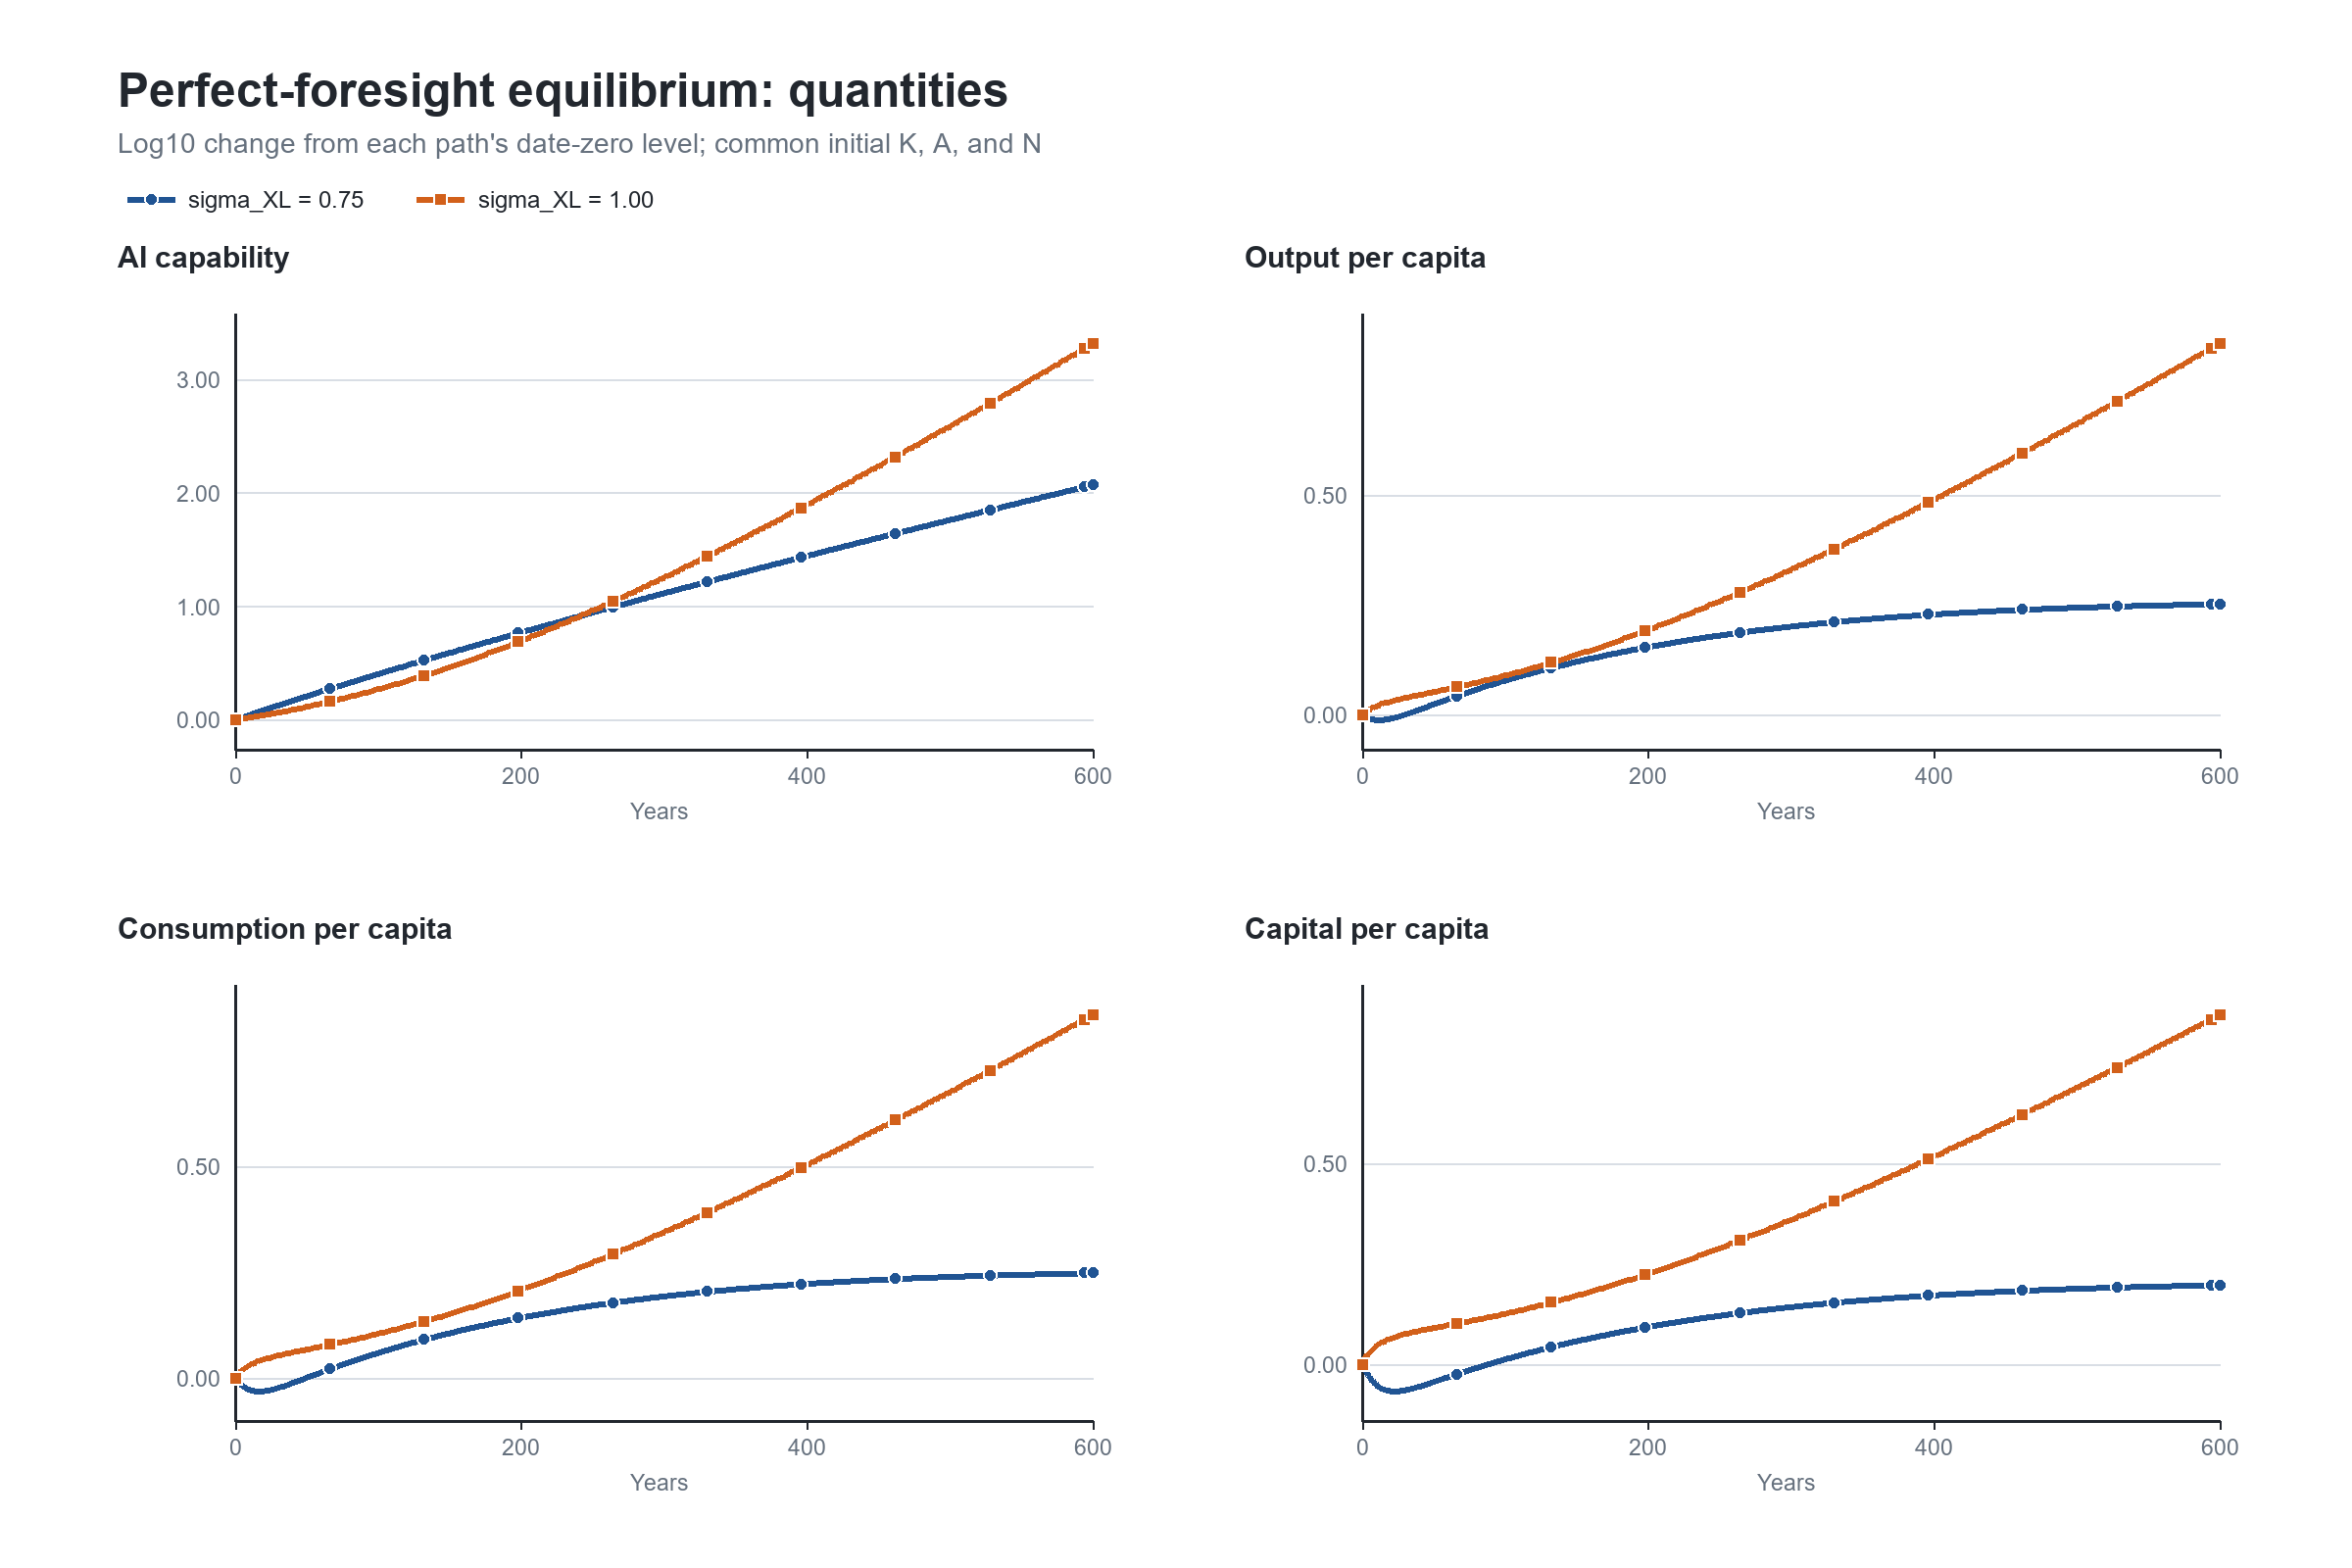
\includegraphics[width=\textwidth]{figures/equilibrium_levels.png}
    \caption{Equilibrium quantities. Each panel reports the base-10 logarithm of
    the change relative to the path's date-zero value. Both paths satisfy the
    household and developer optimality conditions.}
    \label{fig:equilibrium-levels}
\end{figure}

Figure~\ref{fig:equilibrium-growth-rates} makes the complementarity result precise.
When $\sigma_{XL}=0.75$, output-per-capita growth is not zero at every date. It is
negative initially, becomes positive during the recovery, and then converges toward
zero. By year 600 it is 0.0056 percent. Capability growth remains positive and is
close to its analytical limit of 0.675 percent. The experiment therefore
illustrates the production bottleneck characterized in Proposition
\ref{prop:nonunit-ces-steady-states}; it does not prove convergence, which follows
only if the required equilibrium limit exists.

The Cobb--Douglas path is different. Capability growth rises from 0.445 percent to
1.716 percent during the first 600 years and reaches 2.271 percent by year 2,000.
Output- and consumption-per-capita growth then approach the analytical value of
0.568 percent. The net return satisfies the Euler equation along both paths. It
converges to 4 percent under complementarity and to 4.568 percent in the
Cobb--Douglas limit.

\begin{figure}[H]
    \centering
    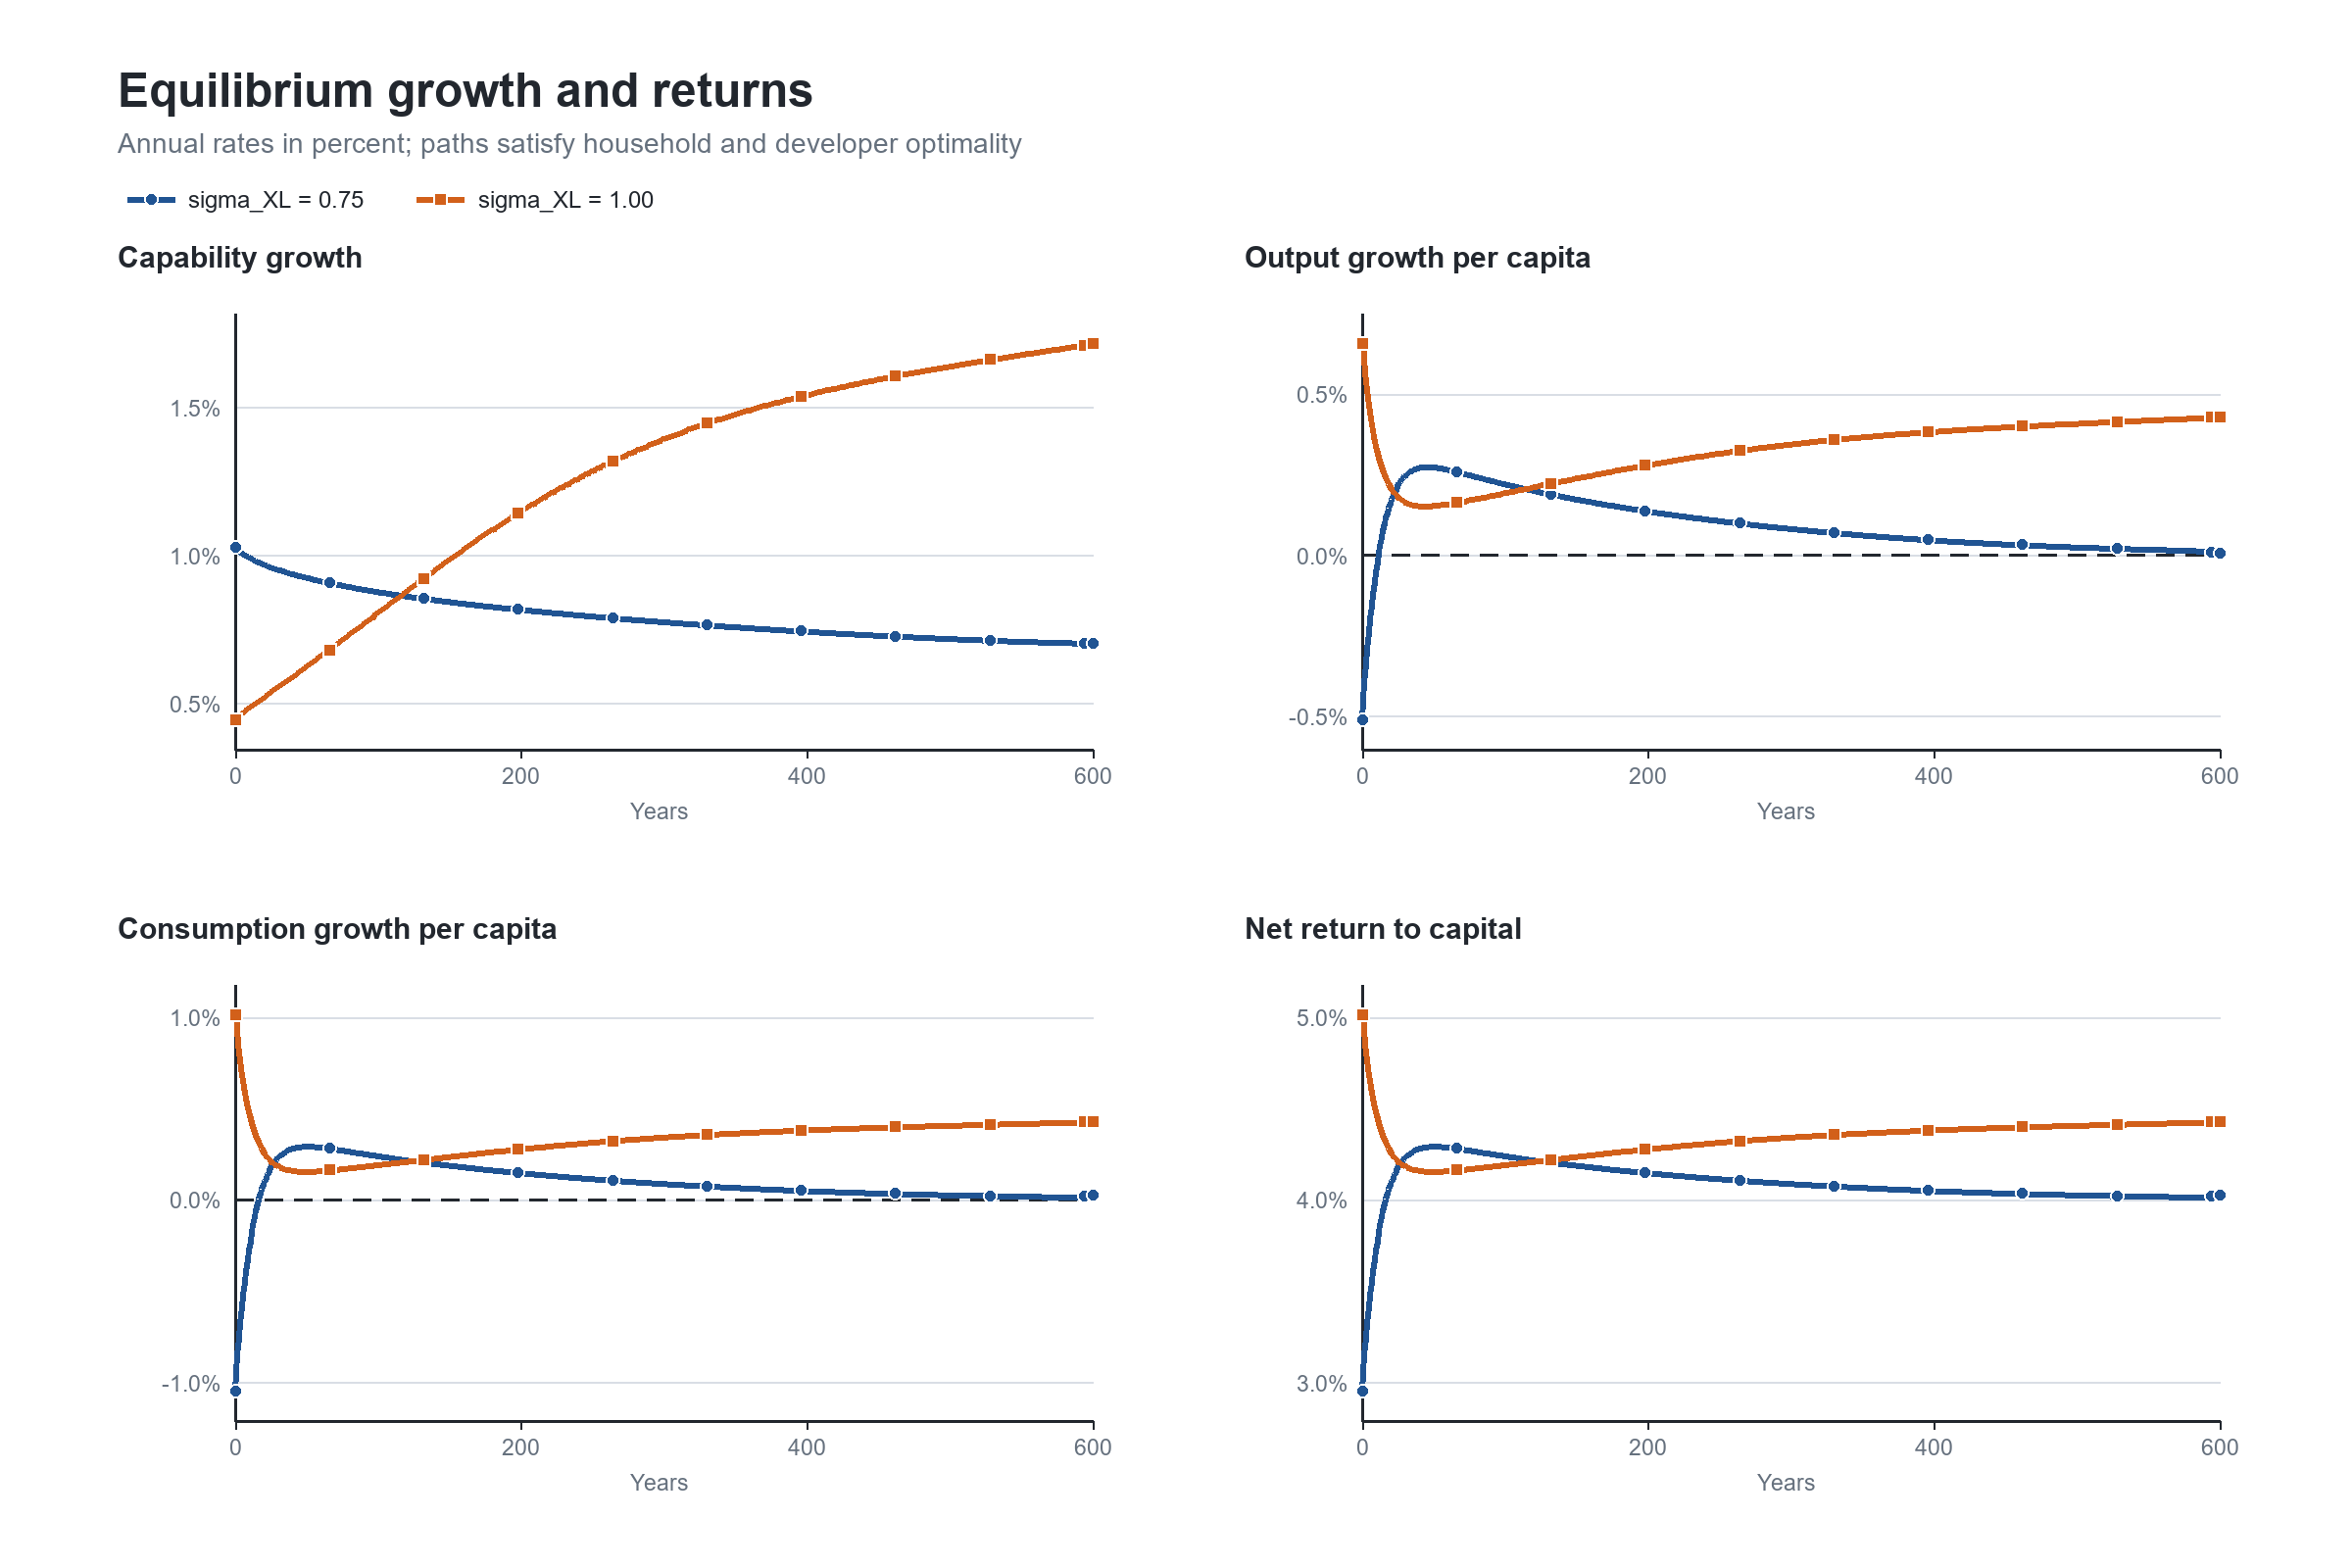
\includegraphics[width=\textwidth]{figures/equilibrium_growth_rates.png}
    \caption{Equilibrium growth rates and the net return to capital. Rates are
    annual. The dashed line marks zero per-capita growth.}
    \label{fig:equilibrium-growth-rates}
\end{figure}

Figure~\ref{fig:equilibrium-factor-shares} reports the allocation of labor and
research. With $\sigma_{XL}=0.75$, the production-labor share rises from 36.05 to
44.46 percent as labor becomes the production bottleneck. The aggregate labor share
rises by almost the same amount because human research employment falls from 1.38
percent to 0.016 percent of the population. The automated contribution to research
increases only from 6.02 to 12.23 percent. A research elasticity above one does not
make automation dominant when the wage remains bounded.

Under Cobb--Douglas production, the production-labor share remains fixed at 53.60
percent. The automated research share rises from 10.60 percent to 45.35 percent by
year 600 and to 99.93 percent by year 2,000. Human research employment is
non-monotone: it rises from 0.19 percent of the population to approximately 0.5
percent and then tends to zero. The development industry can therefore expand its
use of human researchers during part of the automation transition even though
human input eventually becomes negligible relative to automated research.

\begin{figure}[H]
    \centering
    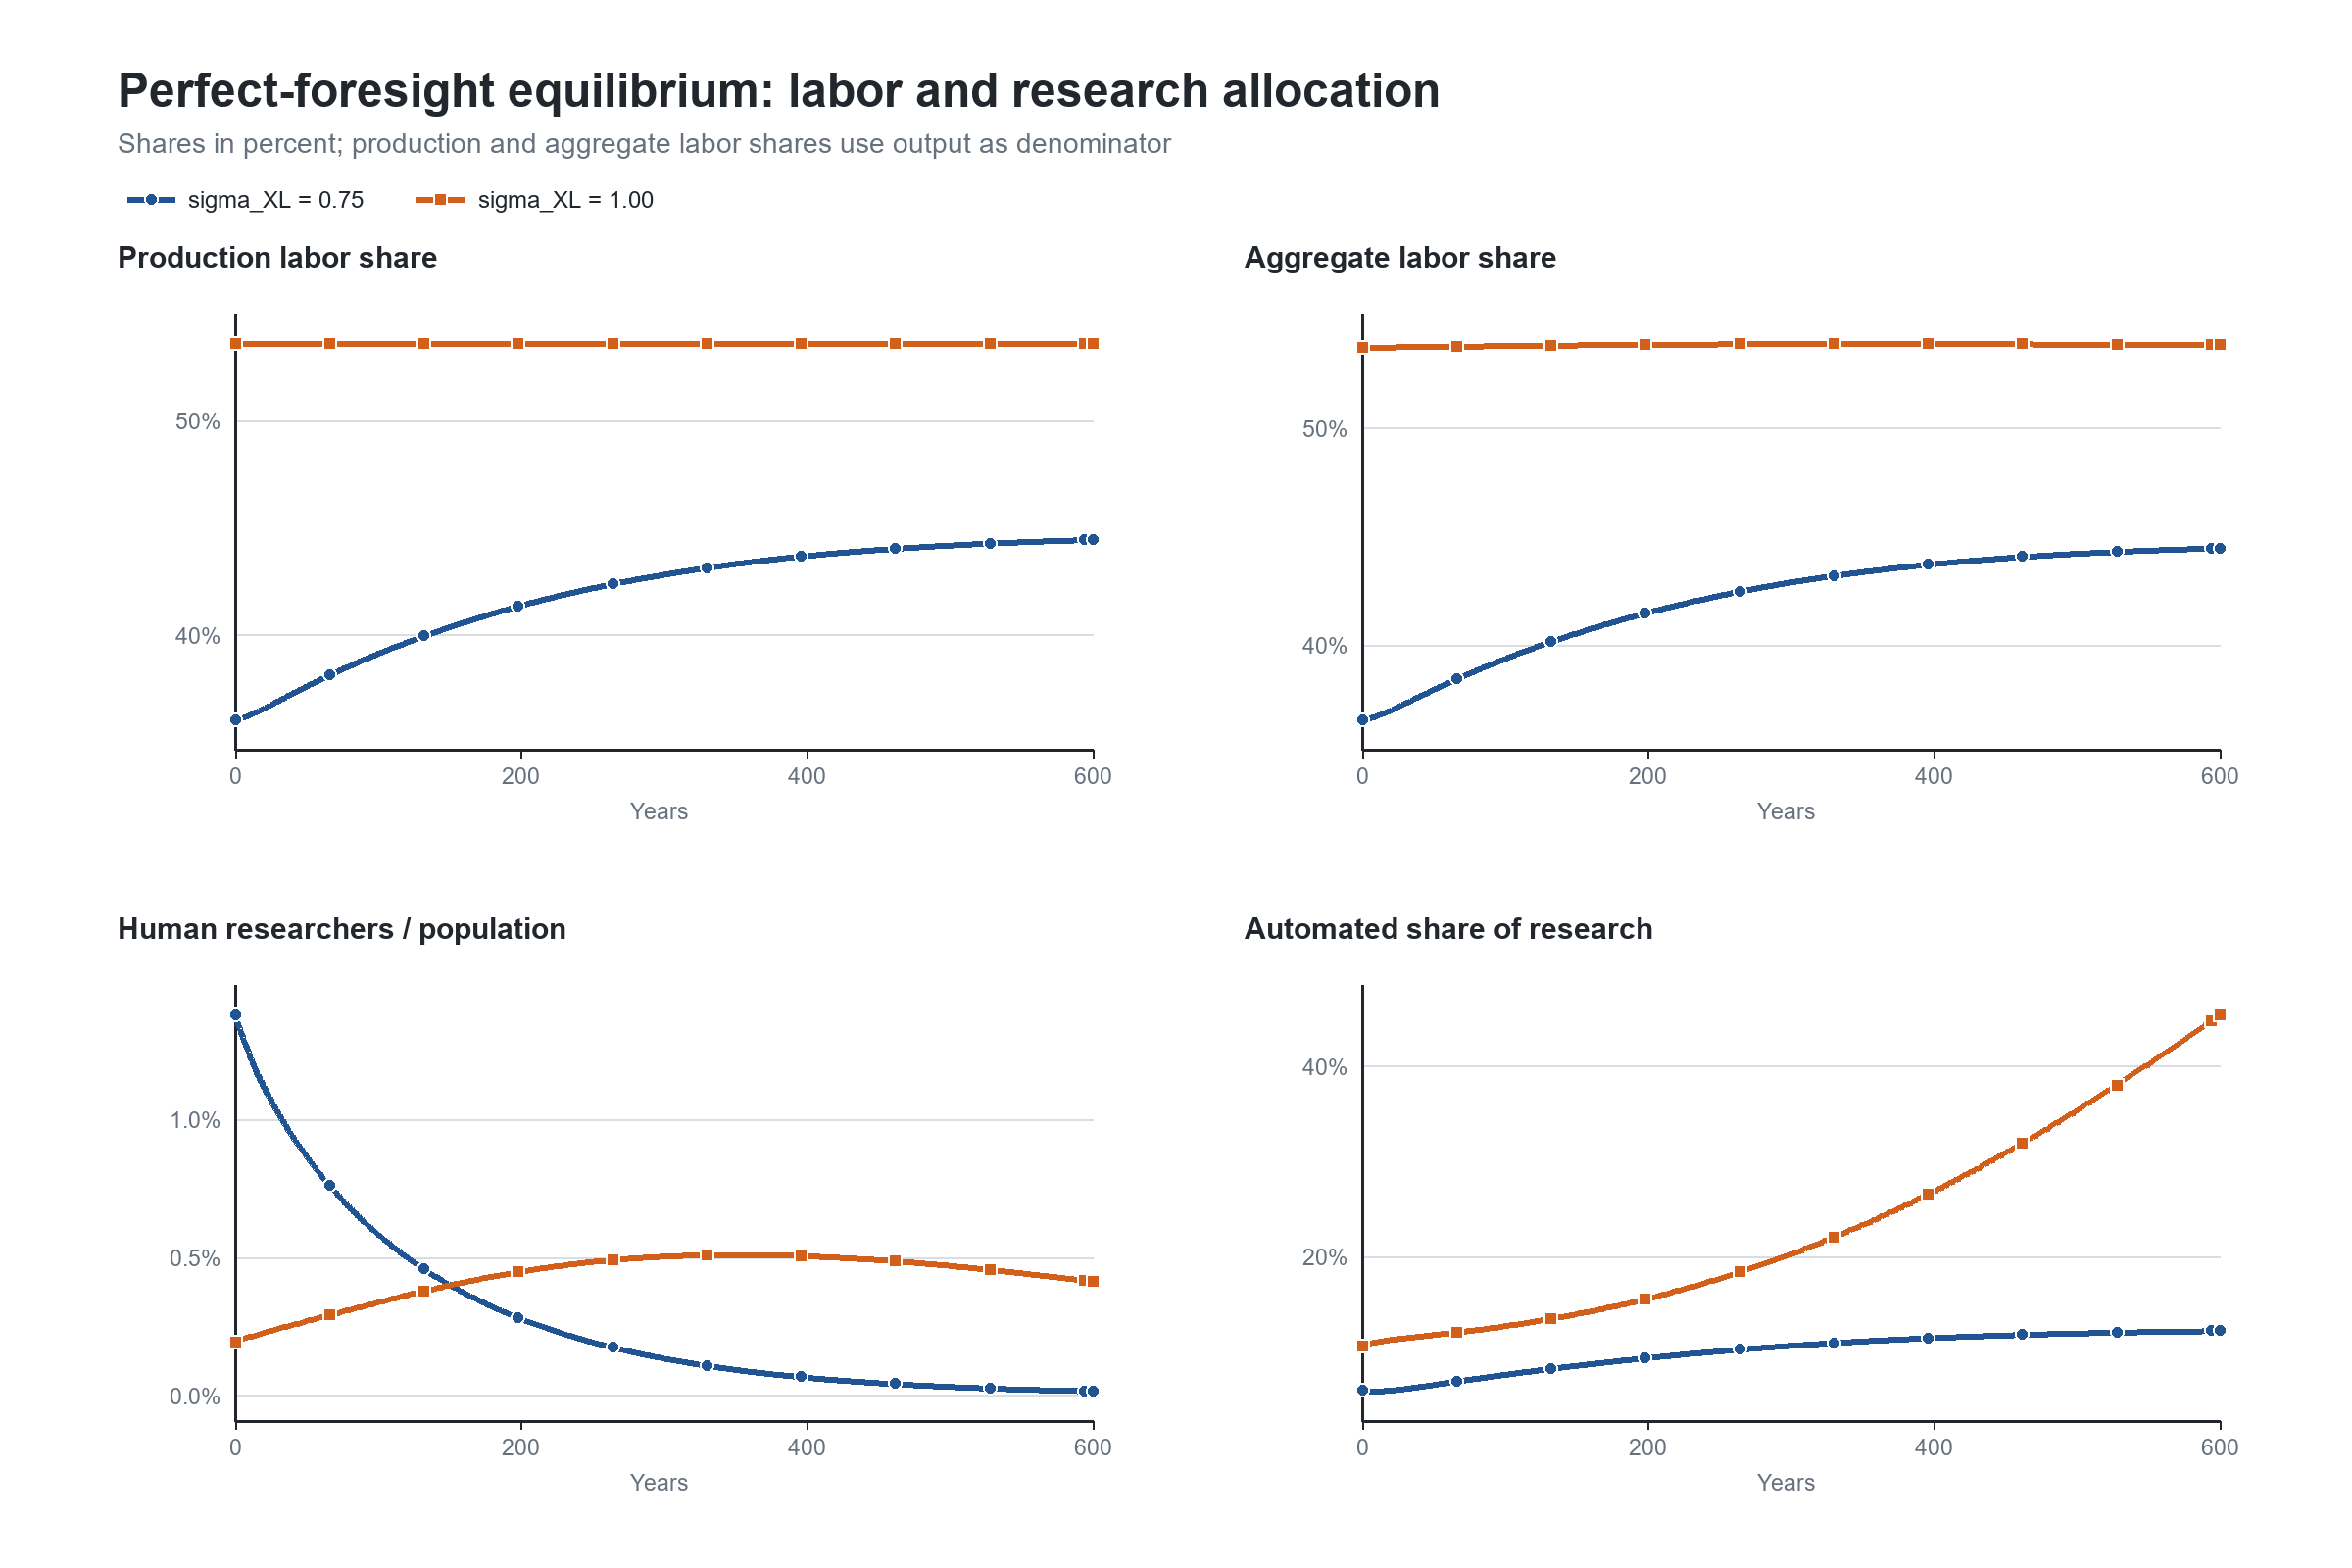
\includegraphics[width=\textwidth]{figures/equilibrium_factor_shares.png}
    \caption{Labor-income shares and the equilibrium research allocation. The
    aggregate labor share includes both production workers and human researchers.}
    \label{fig:equilibrium-factor-shares}
\end{figure}

\subsection{Gross substitution and equilibrium acceleration}

The free-boundary solutions use $\sigma_{XL}=1.35$, $1.50$, and $2.00$. All
three values lie below the static wage threshold $1/\alpha$. This restriction
makes the direct effect of an AI-service expansion on the wage positive, but does
not by itself determine the equilibrium wage path. The simulations verify that the
wage rises and automated research becomes asymptotically dominant. Table
\ref{tab:high-sigma-equilibrium-summary} reports the terminal boundary, the
endogenous time at which the path reaches it, and
\begin{equation}
    \widehat T^*
    =
    T+\frac{1}{\vartheta\bar a\,z_T},
    \label{eq:estimated-singularity-time}
\end{equation}
which follows from equation~\eqref{eq:high-sigma-time-to-singularity}. The final
column reports the smallest wage-growth rate along each path, not its terminal
value.

\begin{table}[htbp]
    \centering
    \caption{Free-boundary equilibrium paths with $\sigma_{XL}>1$}
    \label{tab:high-sigma-equilibrium-summary}
    \begin{tabular}{cccccc}
        \toprule
        $\sigma_{XL}$ & $z_T$ & $T$ & $\widehat T^*$
        & first year $g_{Y/N}\geq5\%$ & $\min_t g_w$ \\
        \midrule
        1.35 & 50  & 333.22 & 333.38 & 297 & 0.070\% \\
        1.50 & 50  & 280.29 & 280.45 & 247 & 0.054\% \\
        2.00 & 100 & 209.00 & 209.08 & 180 & 0.028\% \\
        \bottomrule
    \end{tabular}
    \begin{minipage}{0.96\textwidth}
    \footnotesize\emph{Notes:} Calendar time is measured from the common initial
    stocks. The dates are conditional on the illustrative parameter values in
    Table~\ref{tab:equilibrium-numerical-parameters}; they are not calibrated
    forecasts.
    \end{minipage}
\end{table}

Figure~\ref{fig:high-sigma-equilibrium-levels} shows a long interval of moderate
growth followed by a sharp acceleration. Moving $\sigma_{XL}$ from 1.35 to 2.00
brings the acceleration forward by more than a century. The comparison is not
generated by different investment or research-spending rules: the household and
the developer optimize along every path.

\begin{figure}[H]
    \centering
    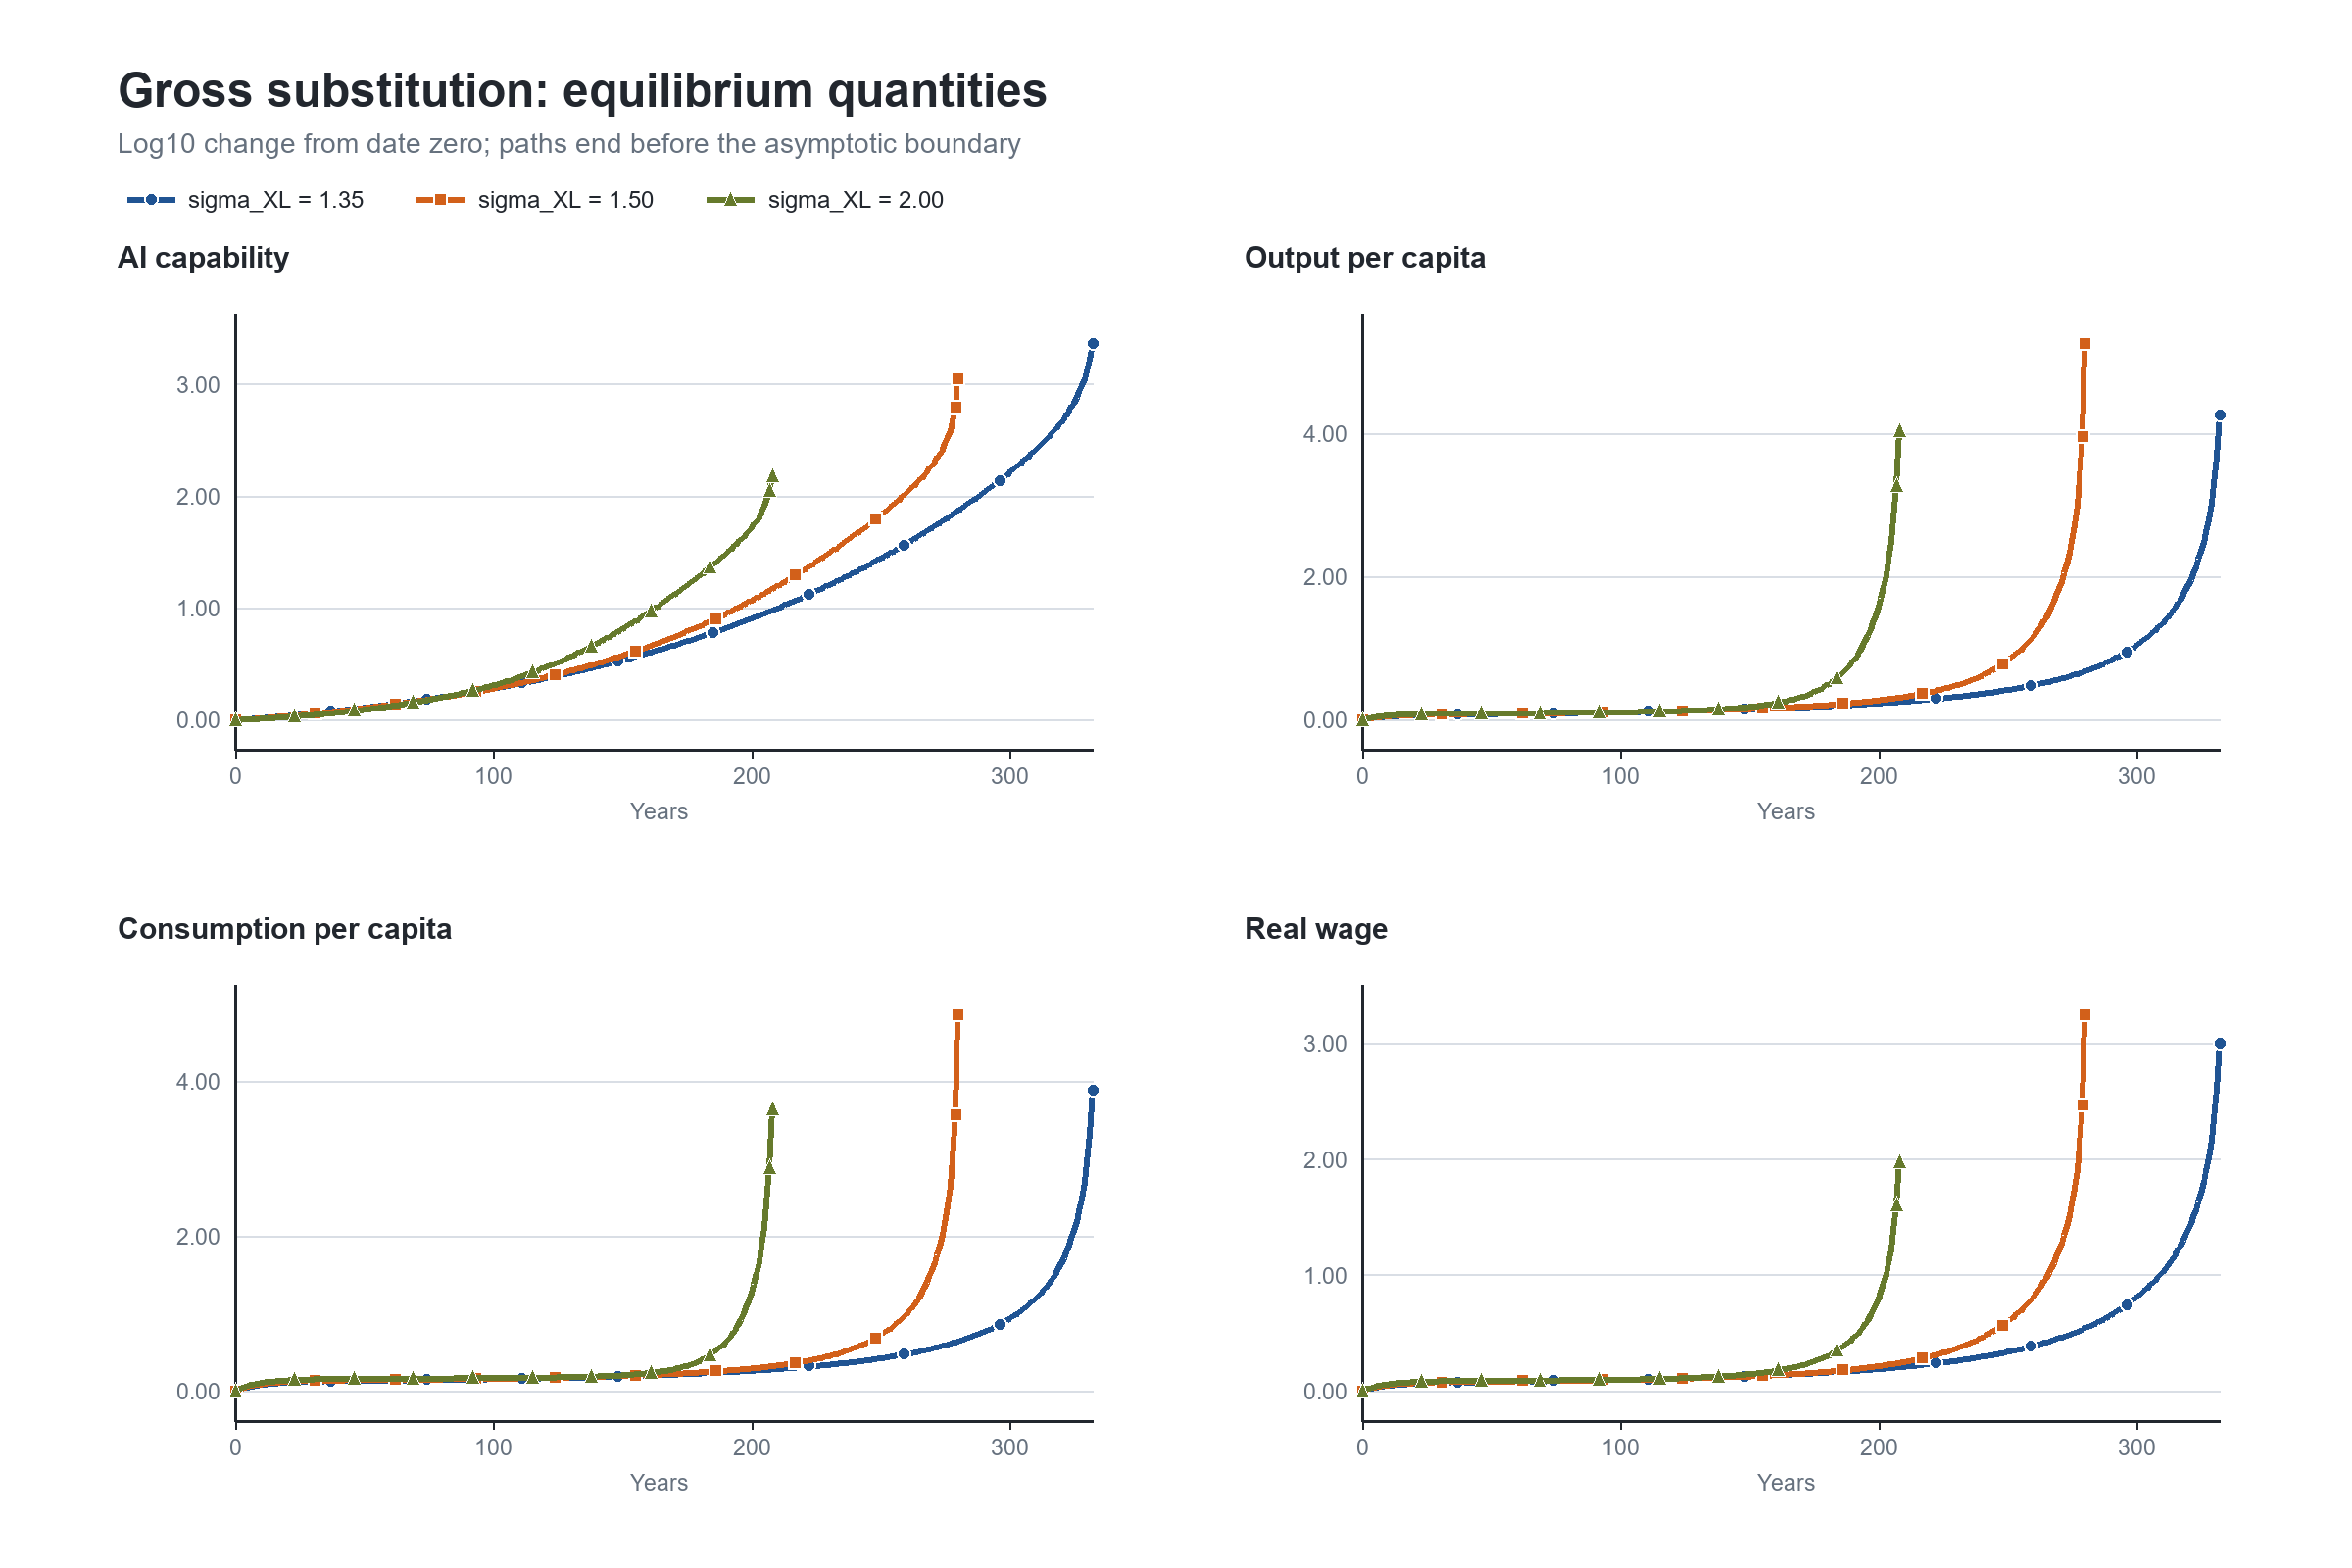
\includegraphics[width=\textwidth]{figures/high_sigma_equilibrium_levels.png}
    \caption{Equilibrium quantities with gross substitution. Each panel reports
    the base-10 logarithm of the change from the path's date-zero value. For
    comparability, the displayed paths end no later than $Y/K=20$.}
    \label{fig:high-sigma-equilibrium-levels}
\end{figure}

The growth rates and the return to capital in Figure
\ref{fig:high-sigma-equilibrium-growth} remain comparatively low through most of
the transition and then rise rapidly. Output-per-capita growth first exceeds 5
percent after 297 years when $\sigma_{XL}=1.35$, after 247 years when it is 1.50,
and after 180 years when it is 2.00. The real wage rises throughout all three
paths. The acceleration therefore does not require a falling wage, even though
labor receives a vanishing share of output.

\begin{figure}[H]
    \centering
    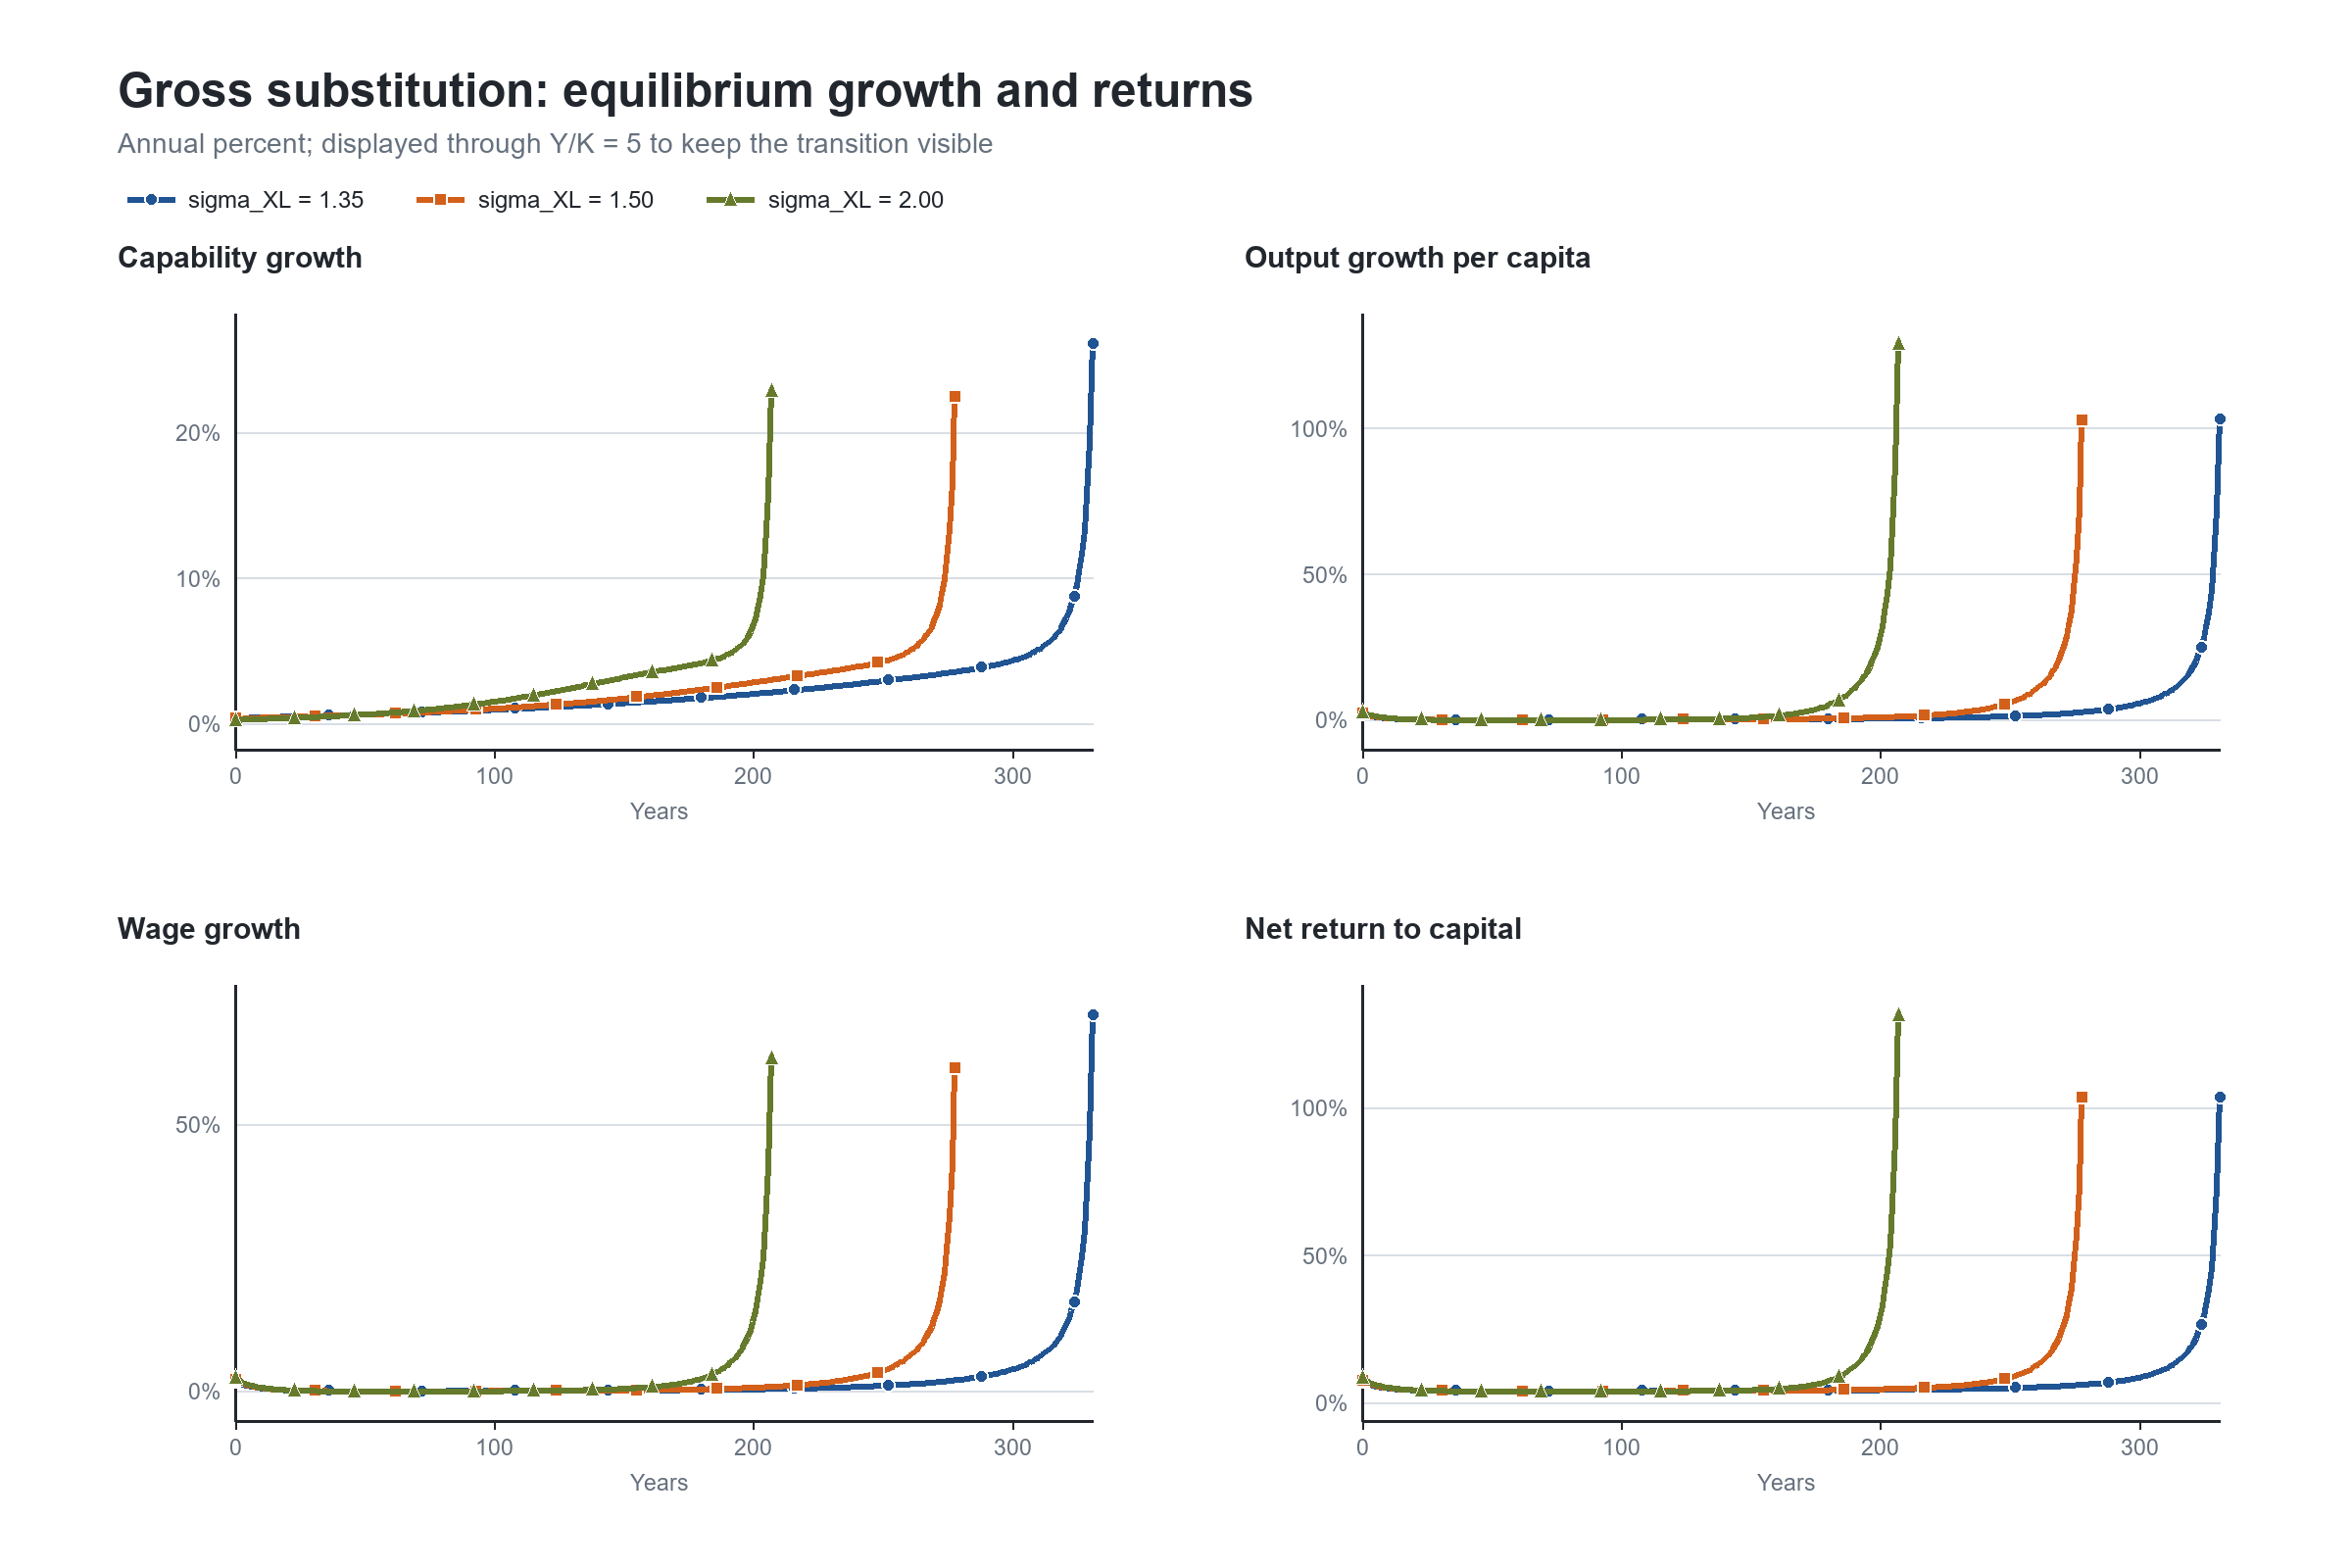
\includegraphics[width=\textwidth]{figures/high_sigma_equilibrium_growth.png}
    \caption{Equilibrium growth rates and net return with gross substitution.
    The figure stops at $Y/K=5$ so that the pre-acceleration transition remains
    visible; output growth and the return to capital diverge subsequently.}
    \label{fig:high-sigma-equilibrium-growth}
\end{figure}

Figure~\ref{fig:high-sigma-equilibrium-shares} separates the production and
research margins. The AI contribution to production and the automated contribution
to research approach one, while the aggregate labor share approaches zero. Human
research employment need not follow the aggregate labor share. With
$\sigma_{XL}=1.35$ and 1.50, $H/N$ rises and later falls as automated research
becomes dominant. With $\sigma_{XL}=2$, the scale of research expands so quickly
that $H/N$ reaches 90.7 percent at the $Y/K=100$ boundary even though automated
systems account for 99.8 percent of effective research. A nearly automated research
technology can therefore employ most humans while paying them a negligible share
of an economy that is growing much faster than wages.

\begin{figure}[H]
    \centering
    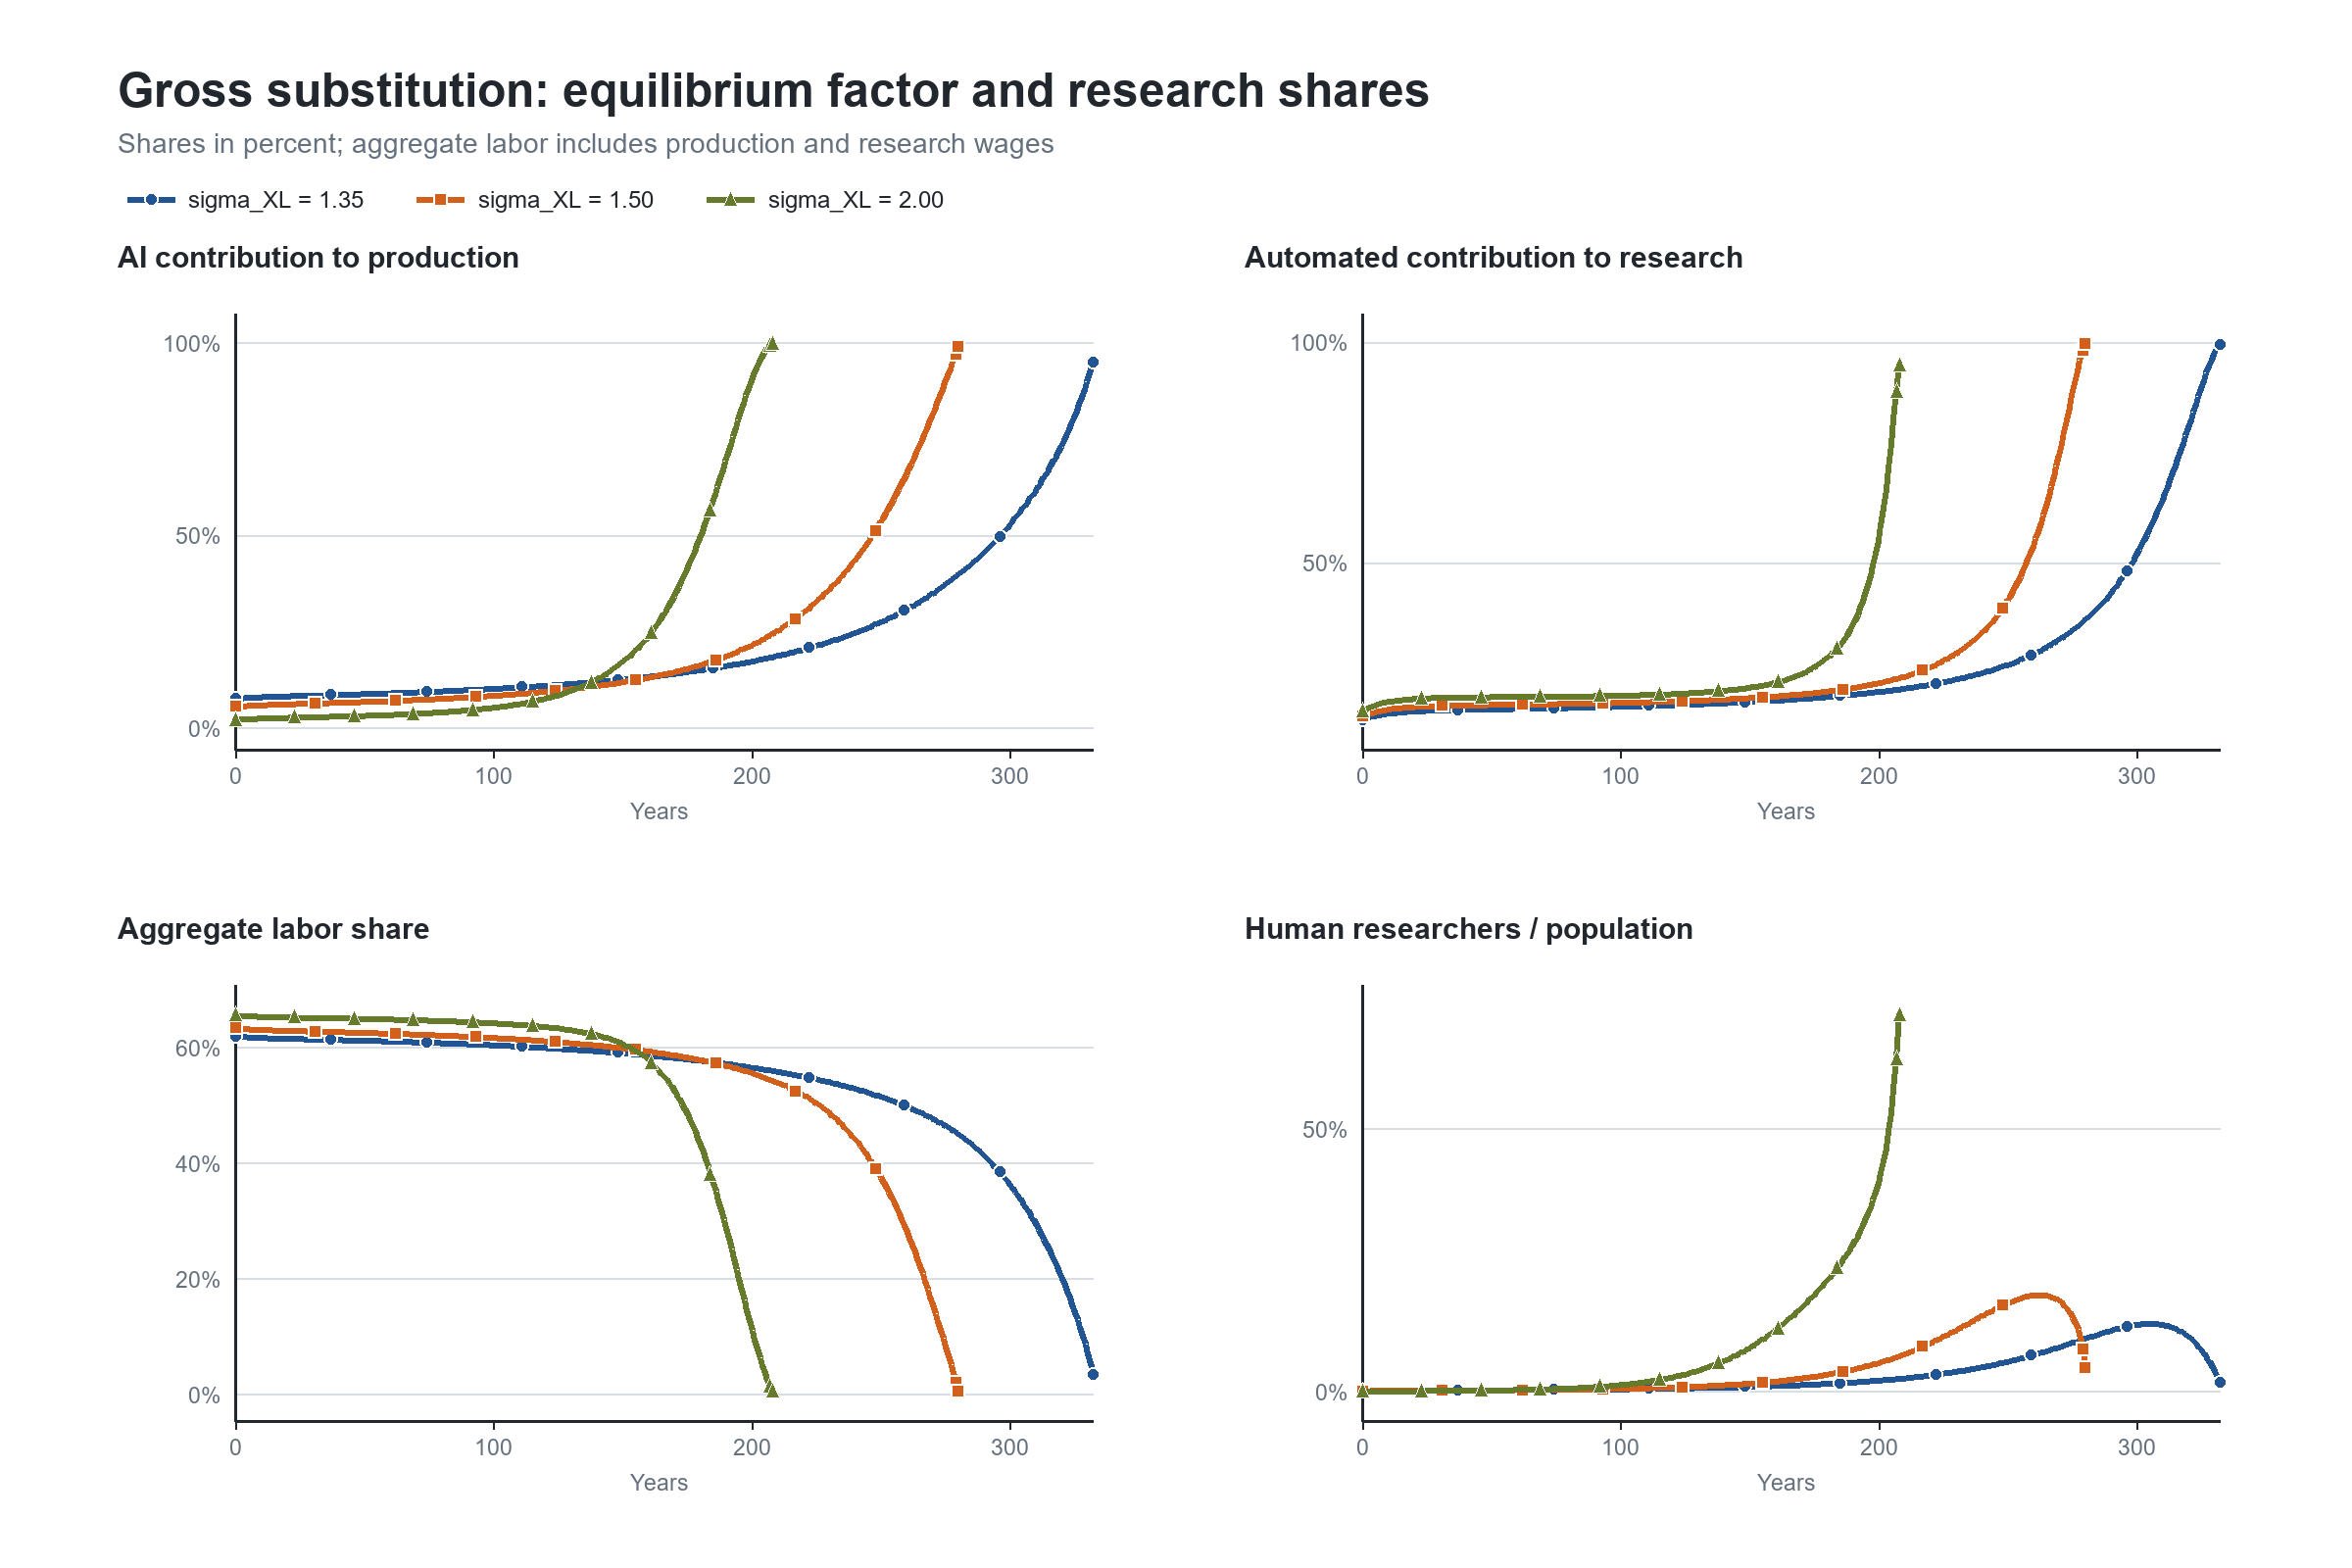
\includegraphics[width=\textwidth]{figures/high_sigma_equilibrium_shares.png}
    \caption{Production, research, and labor allocation along the gross-substitution
    equilibria. The aggregate labor share includes production and research wages.}
    \label{fig:high-sigma-equilibrium-shares}
\end{figure}

The boundary tests show that the terminal condition is not driving the transition.
Moving $z_T$ from 20 to 50 changes $\widehat T^*$ from 333.343 to 333.379 years
when $\sigma_{XL}=1.35$ and from 280.436 to 280.450 years when it is 1.50. For
$\sigma_{XL}=2$, moving $z_T$ from 20 to 50 and then to 100 changes
$\widehat T^*$ from 209.079 to 209.076 and 209.075 years. Across these sequences,
initial log consumption changes by less than $2.1\times10^{-8}$ and the initial log
shadow value by less than $3.0\times10^{-5}$.

The boundary directly imposes $C/Y=26.29$ percent and the limiting value of
$qA/K$. Those two ratios are therefore not independent numerical tests of
Proposition~\ref{prop:high-sigma-singular-scaling}. The non-imposed ratio
$g_A/(Y/K)$ approaches its theoretical value of 0.0624. At the largest boundaries,
the investment shares lie between 20.43 and 20.49 percent, compared with the
predicted 20.33 percent, while automated-research resource shares lie between 8.38
and 9.00 percent, compared with the predicted 8.49 percent. These independent
objects provide the relevant numerical check of the singular scaling.

\begin{figure}[H]
    \centering
    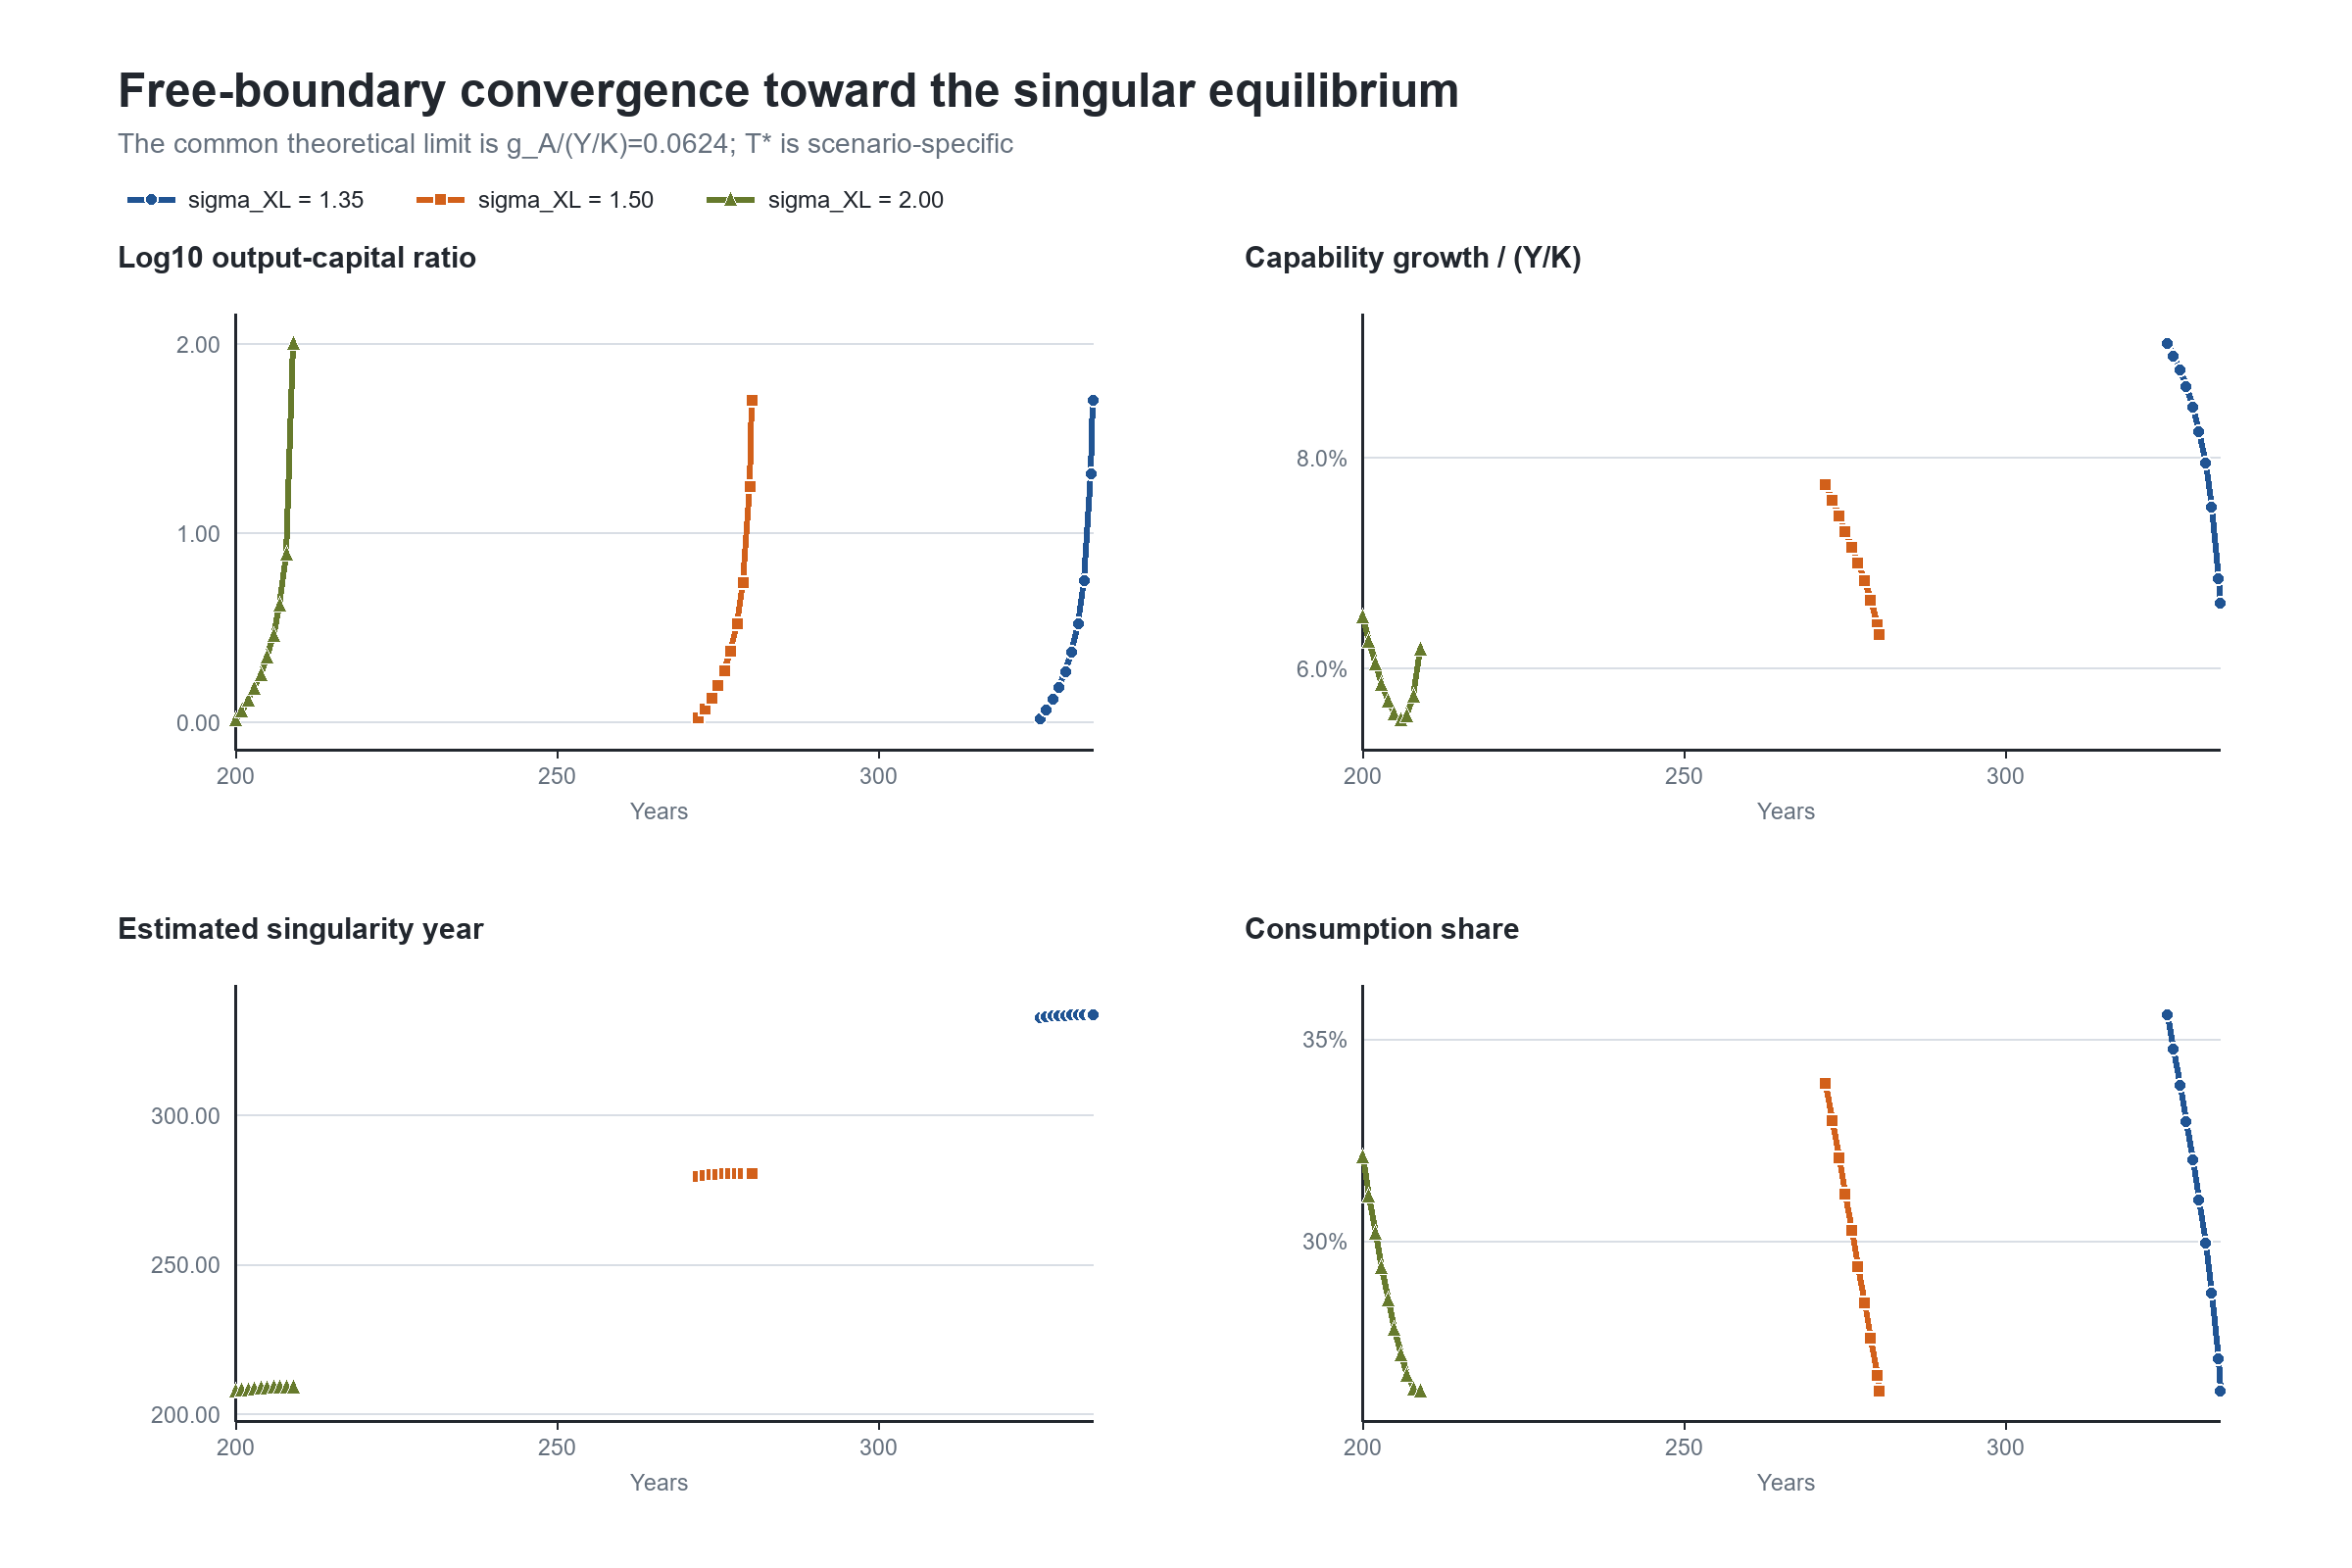
\includegraphics[width=\textwidth]{figures/high_sigma_equilibrium_asymptotics.png}
    \caption{Convergence toward the conditional singular-equilibrium ratios. The
    singularity-date estimator is evaluated only after $Y/K$ reaches one. The
    terminal consumption share is imposed by the free-boundary condition and is
    shown to describe the transition, not as an independent validation moment.}
    \label{fig:high-sigma-equilibrium-asymptotics}
\end{figure}

The maximum collocation residual across the three high-substitution solutions is
$3.0\times10^{-5}$. The largest equation-specific dynamic residual is
$1.7\times10^{-5}$, and the largest static first-order-condition residual is below
$2.0\times10^{-10}$. Labor-market clearing and the aggregate resource constraint
hold to machine precision. These checks establish that the reported curves solve
the numerical equilibrium system on their finite domains. They do not prove global
existence or uniqueness of the limiting singular path.

\subsection{Reassessment of the analytical results}

The audit changes the evidentiary status of several claims, even where it does not
change their mathematical content.
\begin{enumerate}[label=(\roman*)]
    \item Propositions~\ref{prop:wage-share-thresholds},
    \ref{prop:dynamic-labor-share}, \ref{prop:gradual-automation}, and
    \ref{prop:research-employment-scale} are algebraic or conditional identities.
    The five paths satisfy those identities. They also illustrate that a rising wage
    can coexist with a falling labor share and that declining human research
    intensity need not imply declining human research employment.
    \item The $\sigma_{XL}<1$ path is consistent with the necessary limiting rates
    in Proposition~\ref{prop:nonunit-ces-steady-states}; the separate horizon test
    shows that its initial jump variables are stable. This is numerical support for
    the characterized limit, not a proof that the limit exists for every initial
    condition.
    \item The $\sigma_{XL}=1$ path approaches the rates in
    Proposition~\ref{prop:ai-dominated-cd-limit} and is likewise stable when the
    terminal horizon is extended. It supports the conditional Cobb--Douglas
    characterization but does not convert its necessary conditions into a general
    existence theorem.
    \item For $\sigma_{XL}>1$, the paths satisfy the hypotheses of
    Proposition~\ref{prop:gross-substitution-no-steady-state} over their computed
    domains and display the predicted rise in $Y/K$, the return, and consumption
    growth. In Proposition~\ref{prop:high-sigma-singular-scaling}, however, $C/Y$
    and $qA/K$ are terminal boundary conditions. Only the convergence of the
    non-imposed ratios and the stability of the initial jumps and estimated boundary
    date constitute independent numerical evidence for the conditional singular
    branch.
    \item Proposition~\ref{prop:singularity-conditions} concerns a reduced
    proportional-allocation closure, while
    Propositions~\ref{prop:sigma-hm-one-high-sigma-xl} and
    \ref{prop:knowledge-wedge} concern counterfactual research technology or the
    planner. The five equilibrium computations do not test those propositions. They
    must stand on their proofs and stated assumptions, not on these figures.
\end{enumerate}

Finally, the residual audit verifies the canonical necessary conditions, not the
developer's global dynamic optimum in
\eqref{eq:developer-market-value-program}. Because the baseline parameters do not
guarantee global concavity, the numerical objects should be interpreted as locally
regular equilibrium branches selected by the stated endpoint conditions. Certifying
global optimality, existence, and uniqueness remains a separate task.

The previous proportional-allocation simulations remain useful for debugging and
for isolating mechanisms, but they cannot establish equilibrium claims. The new
paths change several quantitative conclusions. Most importantly, the optimizing
developer does not maintain a fixed research-spending share under complementarity,
and the household adjusts saving so that the return to capital and consumption
growth satisfy the Euler equation at every date. Any future numerical extension,
including a wage-decline case with $\sigma_{XL}>1/\alpha$, must meet the same
standard before it is included in the paper.
